\section{液柱垮塌——实验对比以及不同粘度}

\begin{frame}
    \frametitle{\secname}
    \framesubtitle{实验对比}
    \begin{figure}[H]
        \centering
        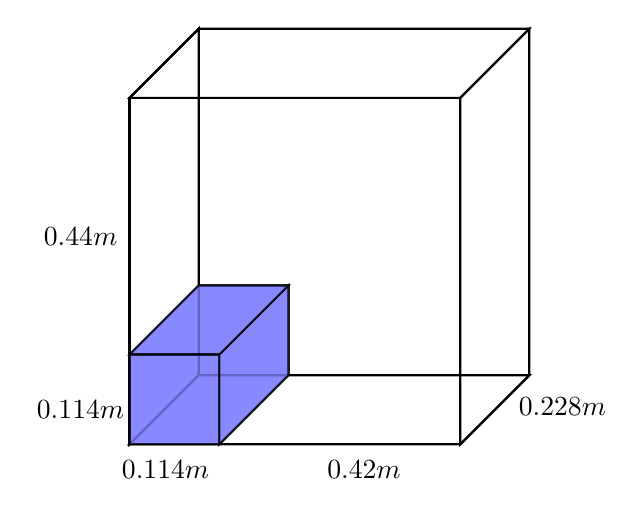
\begin{tikzpicture}
            % a box in 3D space
            % 0.42 width
            % 0.44 height
            % 0.228 depth
            \def\x{0.42*10}
            \def\y{0.44*10}
            \def\z{0.228*10}
            \draw[thick] (0,0,0)--(\x,0,0)--(\x,\y,0)--(0,\y,0)--cycle;
            \draw[thick] (0,0,0)--(0,0,\z)--(0,\y,\z)--(0,\y,0)--cycle;
            \draw[thick] (0,0,0)--(\x,0,0)--(\x,0,\z)--(0,0,\z)--cycle;
            \draw[thick] (\x,0,0)--(\x,\y,0)--(\x,\y,\z)--(\x,0,\z)--cycle;
            \draw[thick] (0,\y,0)--(\x,\y,0)--(\x,\y,\z)--(0,\y,\z)--cycle;
            \draw[thick] (0,0,\z)--(\x,0,\z)--(\x,\y,\z)--(0,\y,\z)--cycle;

            % draw water column
            % initial size is 0.114*0.114*0.228
            % from (0, 0, 0)
            \def\waterx{0.114*10}
            \def\watery{0.114*10}
            \def\waterz{0.228*10}
            \draw[thick,fill=blue!50, opacity=0.75] (0,0,0)--(\waterx,0,0)--(\waterx,\watery,0)--(0,\watery,0)--cycle;
            \draw[thick,fill=blue!50, opacity=0.75] (0,0,0)--(0,0,\waterz)--(0,\watery,\waterz)--(0,\watery,0)--cycle;
            \draw[thick,fill=blue!50, opacity=0.75] (0,0,0)--(\waterx,0,0)--(\waterx,0,\waterz)--(0,0,\waterz)--cycle;
            \draw[thick,fill=blue!50, opacity=0.75] (\waterx,0,0)--(\waterx,\watery,0)--(\waterx,\watery,\waterz)--(\waterx,0,\waterz)--cycle;
            \draw[thick,fill=blue!50, opacity=0.75] (0,\watery,0)--(\waterx,\watery,0)--(\waterx,\watery,\waterz)--(0,\watery,\waterz)--cycle;
            \draw[thick,fill=blue!50, opacity=0.75] (0,0,\waterz)--(\waterx,0,\waterz)--(\waterx,\watery,\waterz)--(0,\watery,\waterz)--cycle;

            % denote the size
            \node at (0.5*\x, -1.2) {$0.42m$};
            \node at (-1.5, 0.4*\y) {$0.44m$};
            \node at (1.1*\x, -0.4) {$0.228m$};
            \node at (-0.1*\x, -1.2) {$0.114m$};
            \node at (-1.5, -0.1*\y) {$0.114m$};
        \end{tikzpicture}
    \end{figure}
\end{frame}

\begin{frame}
    Cruchaga, 2007所做的实验图片,
    原文基于界面捕捉的 FEM。
    \begin{figure}[H]
        \centering
        \includegraphics[width=0.5\textwidth]{images/Cruchaga/cruchaga_experiment.png}
    \end{figure}
\end{frame}

\begin{frame}
    \begin{figure}[H]
        \centering
        \includegraphics[width=\textwidth]{images/Cruchaga/2d/cruchaga_2d.png}
    \end{figure}
    因为差别不大所以只展示不垫高壁面粒子的情形动画。
\end{frame}

\begin{frame}
    同时我还计算了三维情形下的液柱垮塌,
    使用了 1.6 万个粒子,大概计算了 1.5 小时。
    就计算结果而言我认为三维的 SPH 和二维的 SPH 差别很大,三维更准。
    同时壁面粘性还是存在问题,有可能是粒子数不够——$20\times 20\times 40$,
    或者壁面摩擦模型有问题。
    另外我还计算了一个很黏的情况,$\mu=8kg/(m\cdot s)$,但和Cruchaga对不上。
    \begin{figure}[H]
        \centering
        \includegraphics[width=\textwidth]{images/Cruchaga/3d/cruchaga_3d.png}
    \end{figure}
\end{frame}